\section{Постановка задачі техніко-економічного аналізу}
У роботі застосовується метод ФВА для проведення техніко-економічного аналізу розробки.

Відповідно цьому варто обирати і систему показників якості програмного продукту. 

Технічні вимоги до продукту наступні:
\begin{itemize}
	\item програмний продукт повинен функціонувати на персональних комп'ю\-терах зі стандартним набором компонент;
	\item забезпечувати високу швидкість обробки великих об'ємів даних у реальному часі;
	\item забезпечувати зручність і простоту взаємодії з користувачем або з розробником програмного забезпечення у випадку використання його як модуля;
	\item передбачати мінімальні витрати на впровадження програмного продукту.
\end{itemize}

\subsection{Обґрунтування функцій програмного продукту}
Головна функція $F_0$ – розробка програмного продукту, який аналізує процес за вхідними даними та будує його модель для подальшого прогнозування. Виходячи з конкретної мети, можна виділити наступні основні функції ПП:
\begin{description}
	\item[$F_1$] вибір мови програмування;
	\item[$F_2$] інтерфейс користувача;
	\item[$F_3$] вибір камери для роботи.
\end{description}


Кожна з основних функцій може мати декілька варіантів реалізації.
\begin{itemize}
\item Функція F1 :
	\begin{enumerate}
		\item мова програмування Python;
		\item мова програмування С++;
	\end{enumerate}
\item Функція F2:
	\begin{enumerate}
		\item інтерфейс користувача, створений на opencv;
		\item інтерфейс користувача як консольний додаток.
	\end{enumerate}
\item Функція F3:
	\begin{enumerate}
		\item проста веб камера;
		\item Intel Realsense F200.
	\end{enumerate}
\end{itemize}

\subsection{Варіанти реалізації основних функцій}
Варіанти реалізації основних функцій наведені у морфологічній карті системи (рис.~\ref{fig:economics_morph}). На основі цієї карти побудовано позитивно-негативну матрицю варіантів основних функцій (таблиця~\ref{tab:economics_positive_negative_matrix}). 

\begin{figure}
	\centering
	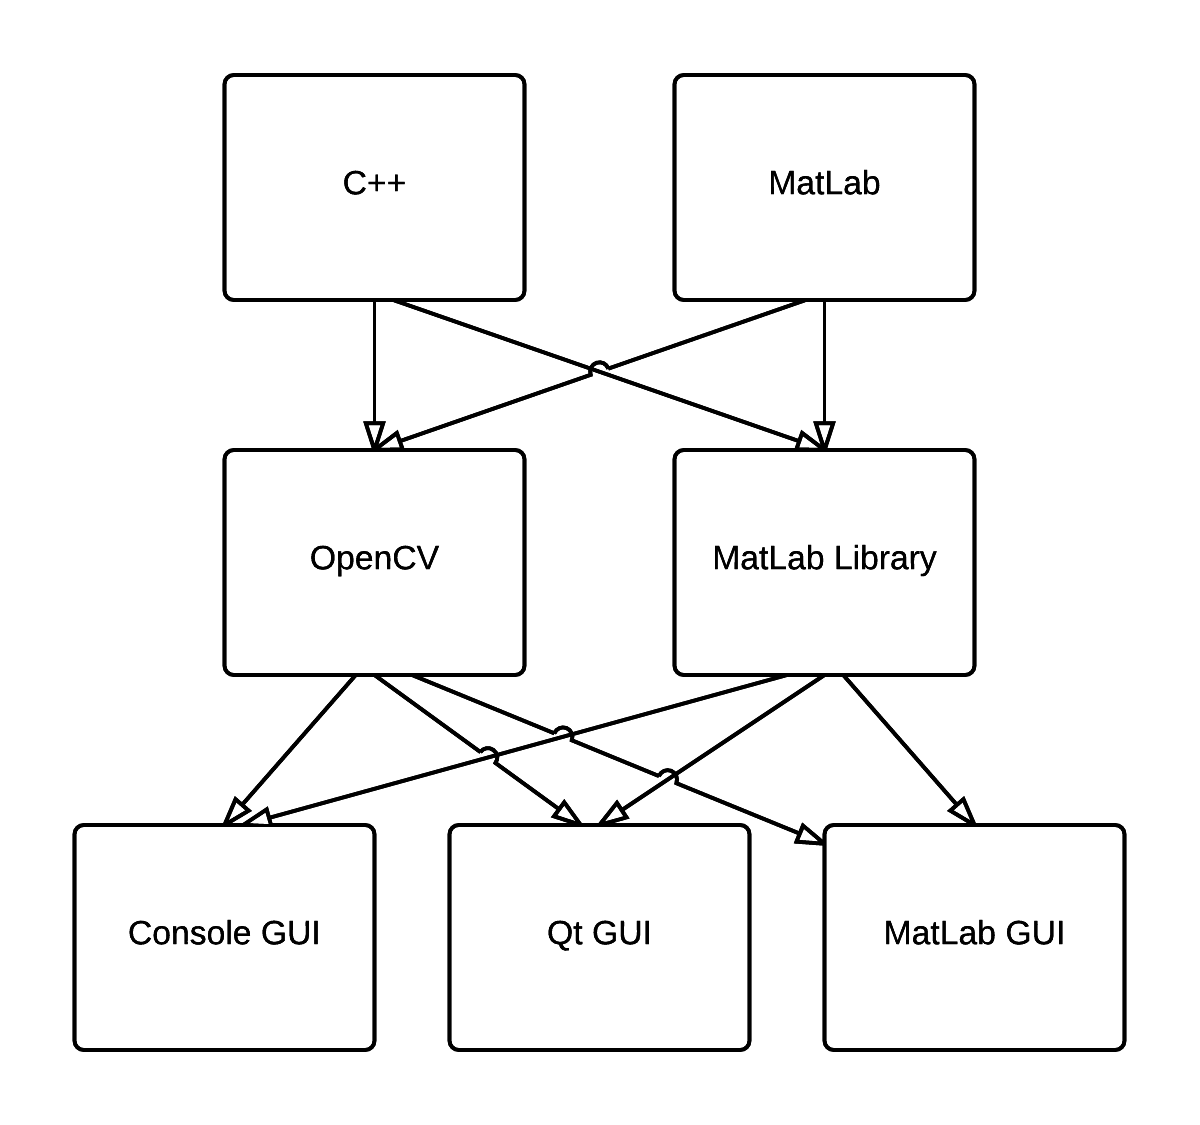
\includegraphics[width=0.7\linewidth]{economics/img/map}
	\caption{Морфологічна карта}
	\label{fig:economics_morph}
\end{figure}


Морфологічна карта відражає всі можливі комбінації варіантів реалізації функцій, які складають повну множину варіантів ПП.

\begin{table}[]
	\caption{Позитивно-негативна матриця}
	\centering
\begin{tabular}{|p{0.12\textwidth}|p{0.13\textwidth}|p{0.3\textwidth}|p{0.3\textwidth}|}\hline
	Основні функції & Варіанти реалізації & Переваги &  Недоліки \\ 
\hline
\multirow{2}{*}{F1}	& А &  Займає менше часу при написанні коду
					& Менша швидкість написання коду \\ 
	 \cline{2-4} 
					& Б & Швидкодійний, кросплатформений
				    & Менша швидкість написання коду\\
\hline
\multirow{2}{*}{F2} & А & Проста розробка 
					& Недостатній функціонал\\ 
	\cline{2-4}         
					& Б & Простота інтерфейса 
					& Неможливість динамічної зміни робочих параметрів \\
\hline
\multirow{2}{*}{F3} & А & Доступність 
					& Лише камера RGB \\
	\cline{2-4}
					& Б & Потужний SDK, depth камера
					& Висока ціна  \\
\hline
	\end{tabular}
	\label{tab:economics_positive_negative_matrix}
\end{table}

На основі аналізу позитивно-негативної матриці робимо висновок, що при розробці програмного продукту деякі варіанти реалізації функцій варто відкинути, тому, що вони не відповідають поставленим перед програмним продуктом задачам. Ці варіанти відзначені у морфологічній карті.
\subsubsection{Функція $F_1$}
Оскільки для нас важлива швидкість роботи, варіант a) має бути відкинутий.
\subsubsection{Функція $F_2$}
\label{subsub:economics_f2}
Оскільки для нас важлива простота, варіант a) має бути відкинутий.
\subsubsection{Функція $F_3$}
Вибір двох різних камер основна ідея проекту і тому вважаємо варіанти a) та b) гідними розгляду.

Таким чином, будемо розглядати такі варіанти реалізації ПП:
\newcommand{\econf}[2]{F_{#1\text{#2} } }
\begin{enumerate}
	\item $\econf{1}{б}$ – $\econf{2}{б}$ – $\econf{3}{а}$
	\item $\econf{1}{б}$ – $\econf{2}{б}$ – $\econf{3}{б}$
\end{enumerate}
Для оцінювання якості розглянутих функцій обрана система параметрів, описана нижче.